\section{Conclusions}
Due to his potential, EternalBlue was implemented in a lot of ransomware like WannaCry. Between 2017
and 2018 the spreading was incredible. Just in 2017 were infected more than 200.000 computers in 150 countries.
Also in Italy there where many cases, in particular part of the network of Milano Bicocca University was compromised.\\
\begin{figure}[ht!]
    \centering
      
\includegraphics[scale=0.3]{images/bicocca.png}
      \caption{Milano Bicocca infected by WannaCry}
\end{figure}

\noindent The National Health Service hospitals in England and Scotland was one of the largest entity compromised by this ransomware. It was particullary 
easy for the ransomware to spread the infection because the file sharing between hospitals was based on the SMB protocol over internet.
\begin{figure}[ht!]
    \centering
      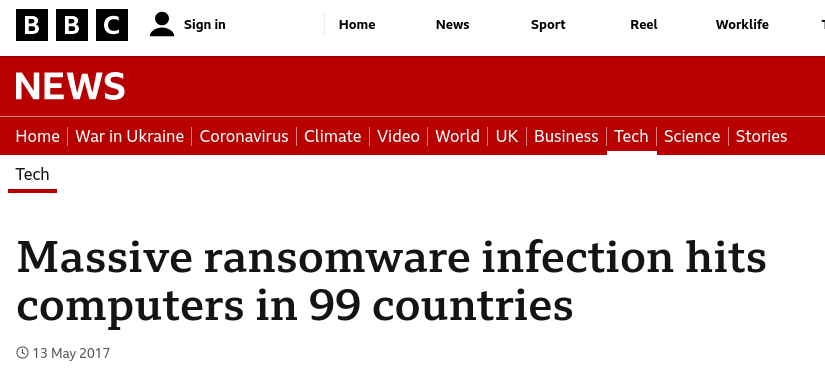
\includegraphics[scale=0.3]{images/bbc.png}
      \caption{BBC article about WannaCry}
\end{figure}

\begin{figure}[ht!]
    \centering
      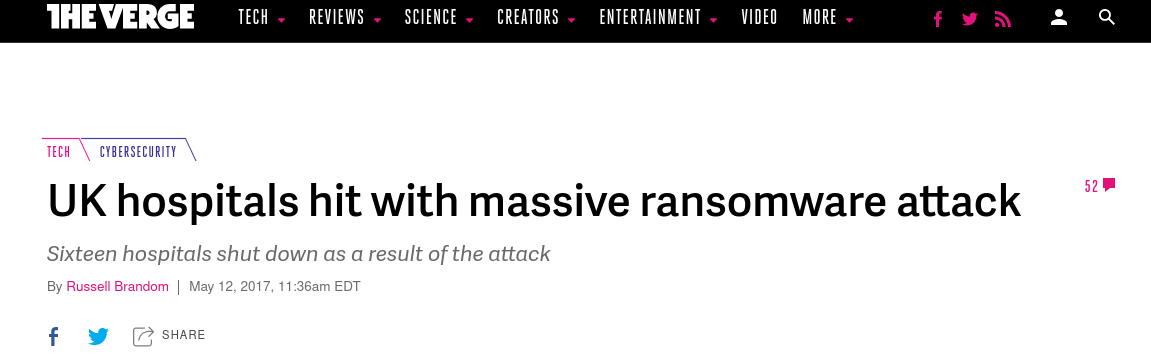
\includegraphics[scale=0.3]{images/theverge.png}
      \caption{The Verge article about WannaCry}
\end{figure}

\noindent Cyence, a cyber risk modeling firm, has estimated the total losses due to WannaCry at \$4 billion, making it one
of the most damaging cyber attack.
